\documentclass[12pt,a4paper]{jarticle}
%
\topmargin=-5mm
\oddsidemargin=-5mm
\evensidemargin=-5mm
\textheight=235mm
\textwidth=165mm
%
\title{''FDPS: A Novel Framework for Developing High-Performance
  Particle Simulation Codes for Distributed-Memory Systems''のメモ}
\author{谷川} \date{}
%\pagestyle{empty}
\usepackage{graphicx}
\usepackage{wrapfig}
\usepackage{lscape}
\usepackage{amssymb}
\usepackage{amsmath}
\usepackage{bm}
\usepackage{setspace}
\usepackage{listings,jlisting}
\usepackage{color}
\usepackage{ascmac}
\usepackage{here}
\usepackage[dvipdfmx]{hyperref}
\usepackage{pxjahyper}

\newcommand{\underbold}[1]{\underline{\bf #1}}
\newcommand{\redtext}[1]{\textcolor{red}{#1}}


%\setcounter{secnumdepth}{4}
%%%%%%%%%%%%%%%%%%%%%%%%%%%%%%%%%%
\setcounter{secnumdepth}{6}
\makeatletter
\newcounter{subsubparagraph}[subparagraph]
\renewcommand\thesubsubparagraph{\thesubparagraph.\@arabic\c@subsubparagraph}
\newcommand\subsubparagraph{\@startsection{subsubparagraph}{6}{\parindent}%
                                       {3.25ex \@plus1ex \@minus .2ex}%
                                       {-1em}%
                              {\normalfont\normalsize\bfseries}}
\newcommand*\l@subsubparagraph{\@dottedtocline{6}{10em}{5em}}
\newcommand{\subsubsubsection}{\@startsection{paragraph}{4}{\z@}%
{1.5\baselineskip \@plus.5\dp0 \@minus.2\dp0}%
{.5\baselineskip \@plus2.3\dp0}%
{\reset@font\normalsize\bfseries}
}
\newcommand{\subsubsubsubsection}{\@startsection{subparagraph}{5}{\z@}%
{1.5\baselineskip \@plus.5\dp0 \@minus.2\dp0}%
{.5\baselineskip \@plus2.3\dp0}%
{\reset@font\normalsize\itshape}
}
\newcommand{\subsubsubsubsubsection}{\@startsection{subsubparagraph}{6}{\z@}%
{1.5\baselineskip \@plus.5\dp0 \@minus.2\dp0}%
{.5\baselineskip \@plus2.3\dp0}%
{\reset@font\normalsize\itshape}
}
\setcounter{tocdepth}{6}
%%%%%%%%%%%%%%%%%%%%%%%%%%%%%%%%%%

%\twocolumn
%\setstretch{1.5}

\lstset{language = C,
numbers = left,
numbersep = 8pt,
breaklines = true,
breakindent = 40pt,
frame = lines,
basicstyle = \ttfamily,
}

\begin{document}
\maketitle
%\tableofcontents

\begin{abstract}

  We have developed FDPS (Framework for Developing Particle
  Simulator), which enables researchers and programmers to develop
  high-performance particle simulation codes easily.  The basic idea
  of FDPS is to separate the program code for complex parallelization
  including domain decomposition, redistribution of particles, and
  exchange of particle information for interaction calculation between
  nodes, from actual interaction calculation and orbital
  integration. FDPS provides the former part and the users write the
  latter. Thus, a user can implement a high-performance N-body code
  only in 120 lines. In this paper, we present the structure and
  implementation of FDPS, and describe its performance on two sample
  applications: gravitational N-body simulation and Smoothed Particle
  Hydrodynamics simulation. Both codes show very good parallel
  efficiency and scalability on the K computer. FDPS lets the
  researchers concentrate on the implementation of physics and
  mathematical schemes, without wasting their time on the development
  and performance tuning of their codes.

  我々は高性能な粒子シミュレーションコードの開発を容易にするフレームワー
  ク「FDPS (Framework for Developing Particle Simulator)」を開発した。
  FDPSの基本的な考えかたは、実際の相互作用計算や軌道積分と、並列化のた
  めの繁雑なプログラム(領域分割、粒子交換、相互作用計算のための粒子情報
  の交換など)を分離することである。FDPSが前者を提供するため、ユーザーは
  後者だけを書けばよい。従って、ユーザーは高性能なN体コードをわずか120
  行で記述できる。この論文では、FDPSの構造とその実装、2つのサンプルア
  プリケーションの性能を示す。どちらのコードも、京コンピュータ上で、良
  い効率とスケーラビリティを示した。FDPSのおかげで、研究者は自分のコー
  ドの開発やチューニングに時間をかける必要がなくなり、物理・数学スキー
  ムの実装に集中することができるようになる。

%%  (ゴードンベルなら以下も記述) 重力N体シミュレーションコードの性能は、
%%  N粒子京コンピュータN ノードで、1ステップあたりX秒で、XFLOPSであっ
%%  た。これは過去のゴードンベル賞の性能値に匹敵する。汎用の粒子シミュ
%%  レーションコードを開発するためのフレームワークでこれを達成したのは
%%  驚くべきことである。また、自己重力SPHシミュレーションコードの性能は、
%%  N 粒子京コンピュータNノード上で、1ステップあたりの時間がX 秒で、
%%  XFLOPSであった。これは広く利用されているXXXコード\{に匹敵する/と比
%%  べてはるかに高性能である\}。

\end{abstract}

%%%%%%%%%%%%%%%%%%%%%%%%%%%%%%%%%%%%%%%%%%%%%%%%%%%%%
\section{Introduction}

この数十年間で、数値シミュレーションは実験、観測、理論による研究手法と
同等の研究手法としての地位を確立した。数値シミュレーションの中でも、粒
子シミュレーションは最も重要なシミュレーション手法の1つである。粒子シ
ミュレーションは、系を粒子の集団とみなし、粒子の運動を追うことで系の進
化を表現する。粒子シミュレーションは様々な理工学の分野で使われていて、
たくさんのアプリケーションがある。例えば、重力$N$体シミュレーション、分
子動力学シミュレーション、粉体シミュレーション、流体力学のためのメッシュ
フリーシミュレーションである。粒子シミュレーションは、格子シミュレーショ
ンに比べて、大きな変形を伴う系を扱うのに有利である。

%%数値シミュレーションは多数回実験を繰り返すよりも安価である。また、宇
%%宙現象のような1度しか起こらない現象を何度もシミュレートすることがで
%%きる。理論研究では物理現象の線形領域までしか追うことができないが、数
%%値シミュレーションではその非線形領域も追うことができ、研究対象を大幅
%%に広げている。

%%SPHシミュレーションやMPSシミュレーション。\redtext{(mesh-based VS
%%meshfree method: handle complex situations such as extremely large
%%deformation of bodies, impact problems, treatment of discontinuities
%%as in multiphases flows, or free surface flows. (Lanson \& Vila
%%2008a))}

時空方向にダイナミックレンジの大きい系の進化を追跡するために、高性能な
粒子シミュレーションの必要性はますます高まっている。
%%より高い空間解像度または質量解像度を実現するために、大粒子数の粒子シ
%%ミュレーションを短時間で実行できるコードへの要請は、枚挙にいとまがな
%%い。また、扱う時間スケールが粒子の力学的時間よりはるかに長いために、
%%少ない粒子数でも高性能に実行できるコードへの要請もある。
しかし、普通の研究者やプログラマーにとってこのような高性能な粒子シミュ
レーションコードを作成するのは難しい。このようなコードは大規模並列分散
メモリ計算機で動作する必要がある。このような計算機で動作するためには、
コードは以下のような処理を備えていなければならない。すなわち、ロードバ
ランスのための動的な領域分割、領域分割に合わせた粒子情報の交換、相互作
用を計算するための粒子情報の交換、である。さらに、研究者やプログラマー
は、共有メモリ環境下でも高性能を達成するために、複数コア、キャッシュメ
モリ、SIMDユニットの効率的な使用を考慮する必要がある。

これまで研究者、プロブラマー、それらのグループは個別にこのようなコード
を開発してきた。しかし、これらのコードの設計、実装、テスト計算、デバッ
グには多大な時間がかかる。そのため、研究者やプログラマーはコード開発に
時間をとられ、理工学の研究に専念できないでいる。

我々は、この状況を打破するために、高性能な粒子シミュレーションコードの
開発を容易にするフレームワーク「FDPS (Framework for Developing
  Particle Simulator)」を開発した。FDPSを使えば、そのユーザーは、分散メ
モリ環境用の繁雑な処理や共有メモリ環境用のチューニングをすることなしに、
高性能な粒子シミュレーションコードを作成できる。ユーザーがすることは、
並列処理を行うFDPSライブラリを呼出すことと、1コア上での粒子間相互作用の
計算と共有メモリ環境での粒子の軌道積分を実装することだけである。FDPSは
すでにGithubに公開されている。
%%FDPSは、物理現象を表現するために必要なプログラム部分を、上に述べた分
%%散メモリ環境における処理や共有メモリ環境におけるチューニングから分離
%%することに成功した。これを実現するために、後者の部分を、C++のテンプレー
%%トクラスを用いて、抽象化した。従って、FDPSは並列処理やチューニングの
%%ための処理を担当し、研究者は物理現象を表現する部分のみ記述することに
%%なる。研究者は粒子シミュレーションコードを高性能にするための作業から
%%解放され、よりクリエイティブな仕事に専念できるようになる。さらに、
%%FDPSを用いて作成された粒子シミュレーションコードは、世界最高レベルの
%%性能を持つことを強調しておく。FDPSは
%%Github\footnote{https://github.com/FDPS/FDPS}に公開済である。

FDPSの特長は、あらゆる粒子シミュレーションコードに対応していることであ
る。これまでに、多くの高性能な粒子シミュレーションコードが開発されてき
た。しかし、それらのコードはアプリケーションが限られていた。N体シミュレー
ションならGreeM、N体+SPHならGadgetやGasoline、などのように。
%%これまで、様々な高性能な粒子シミュレーションコードが開発されてきた
%%(GreeM, Gadget, gasoline, PAM-CRASH, PPPP, etc)。しかし、それらは特定
%%のアプリケーションに限られていた。FDPSは任意の粒子シミュレーションコー
%%ドを開発することが可能であることに大きな利点がある。

この論文の構成は以下の通りである。2節では、FDPSを使った粒子シミュレーショ
ンコードの実装方法を概観し、ユーザーが高性能化をする必要がないことを示
す。3節では、FDPSの中の実装を記述する。4節では、FDPSのアプリケーション
として重力N体シミュレーションとSPHシミュレーションの性能を示す。これら
のシミュレーションは科学的に重要な意義のあるものである。5節ではこの論文
をまとめる。

\section{FDPSを使った粒子シミュレーションコードの実装}

この節では、FDPSを使った粒子シミュレーションコードの実装方法を記述する。
2.1節では、実装方法を概観し、高性能化に伴う実装がユーザーから分離されて
いることを確認する。2.2節では、サンプルコードを示し、実装方法を詳述する。

\subsection{概観}

粒子シミュレーションコードは以下のような常微分方程式を解くために実装さ
れるものである。
\begin{align}
  \frac{d\bm{u}_i}{dt} = \sum_{j}^N \bm{f}(\bm{u}_i,\bm{u}_j) +
  \bm{g}(\bm{u}_i) \label{eq:geq}
\end{align}
ここで、$N$は全粒子の個数、$\bm{u}_i$は$i$粒子の物理量を表すベクトル、
関数$\bm{f}$は$j$粒子から$i$粒子への作用を表す関数、関数$\bm{g}$は$i$粒
子自身の物理量だけで決まる作用(外場など)である。

\begin{figure}
  \begin{center}
    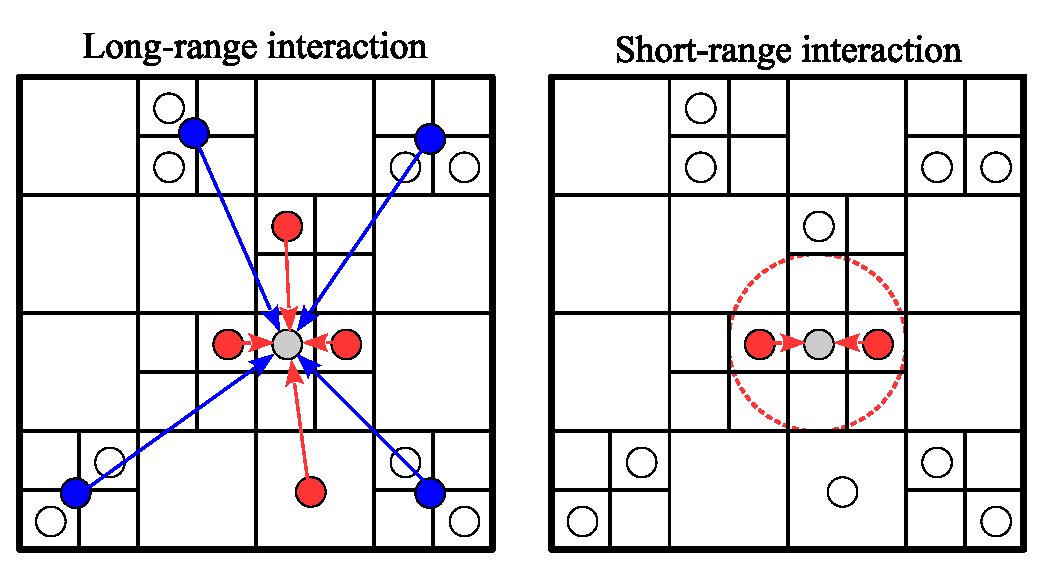
\includegraphics[width=8cm]{fig/force_type.eps}
  \end{center}
  \caption{長距離力と短距離力}
  \label{fig:force_type}
\end{figure}

空間分割を必要に応じて動的に分割し、粒子を再配置する。

この3つに分けて上の2つはFDPSを呼出す。

メインルーチンで実行される処理は、1タイムステップにつき、以下のように
なっている。
\begin{enumerate}
\item FDPSのAPIを呼出してロードバランスをとる。式(\ref{eq:geq})で言えば、
  どのプロセスがどの$i$粒子の方程式を時間積分するかを決めることである。
  ロードバランスは以下のサブステップに分かれている。
  \label{proc:loadbalancing}
  \begin{enumerate}
  \item 粒子の空間分布を反映させて、計算領域を分割する。各プロセスが担
    当する空間領域を決める。その空間領域にある粒子はそのプロセスが担当
    する。これは上で定義した粒子クラスを受け入れるテンプレートライブラ
    リのAPI を呼出すことで実行される。
    \label{proc:decomposeDomain}
  \item 粒子情報の交換。自分の担当する空間領域に存在する粒子の情報を得
    るために、他のプロセスと粒子情報の交換をする。これは上で定義した粒
    子クラスを受け入れるテンプレートライブラリのAPIを呼出すことで実行さ
    れる。
    \label{proc:exchangeParticle}
  \end{enumerate}
\item FDPSのAPIを呼出して相互作用を計算する。上の方程式で言えば、
  $\sum$内を計算することである。この作業は、$\sum$内を計算するのに、必
  要な粒子情報を他のプロセスから受け取るという処理が必要となる。これは、
  上で定義した粒子クラスと相互作用関数を受け入れるテンプレートライブラ
  リのAPIを呼出すことで実行される。
  \label{proc:calcInteraction}
\item プロセス内の情報だけで閉じた計算をする。上の方程式で言えば、
  $\bm{g}(\bm{u}_i)$の計算をすることや、$d\bm{u}_i/dt$を使って時間積分
  をすることである。これは自分で記述する。 \label{proc:local}
\end{enumerate}

FDPSユーザーは、粒子シミュレーションコードを実装するときに以下の3つを
行うことになる。
\begin{itemize}
\item 粒子を定義する。これはある1つの粒子がどのような情報を持つかを決
  めることであり、式(\ref{eq:geqLong})や(\ref{eq:geqShort})の物理量ベク
  トル$\bm{u}_i$や$\bm{\hat{u}}_s$の中身を決めることに対応する。
  $\bm{u}_i$の中身には、例えば、粒子の質量、位置、速度、加速度などがあ
  る。これはC++のクラスという形で定義する。
\item 相互作用を定義する。相互作用の定義とは、2つの粒子の間に働く相互
  作用の形を決めることであり、式(\ref{eq:geqLong})や
  (\ref{eq:geqShort})の関数$\bm{f}$、$\bm{\hat{f}}$を決めることに対応す
  る。これはC++の関数オブジェクトという形で定義をする。
\item メインルーチンを作成する。メインルーチンの中の並列処理は、FDPSが
  提供するテンプレートライブラリのAPIを呼出すことで実行される。このテン
  プレートライブラリは上で定義した粒子と相互作用を受け入れる形になって
  いる。
\end{itemize}
これを概念図として書くと図\ref{fig:concept}のようになる。

上で示した手順のように、ユーザーは並列処理をFDPSが提供するテンプレート
ライブラリのAPIを呼出すことで実行できる。そのため、ユーザーは並列処理の
実装に頭を悩ます必要がない。ユーザーがメインルーチンの中で記述すべき部
分は、時間積分などのプロセス内の情報だけで閉じた処理だけである。

粒子を集めるときには、ツリーアルゴリズムが使われて、高速になされるが、
ユーザーはツリーを実装する必要はないし、意識する必要もない。

式(\ref{eq:geq})の第1項は、全粒子からの$i$粒子への作用を計算するという
ことを示す。しかし、実際には、全粒子の数よりもはるかに少ない粒子からの
相互作用しか計算しない。これはFDPS内部で以下のような実装をしているから
である。FDPSは相互作用を2つのタイプにわけ、1つを無限遠まで到達する長
距離力、もう1つを有限の距離しか到達しない短距離力とした。長距離力の場
合には、ツリーアルゴリズムを用いて、遠くの複数の粒子を1つの超粒子とし
てまとめる(図\ref{fig:force_type}の左)ため、計算する相互作用の数はNより
はるかに少くなる。従って、FDPSでは、長距離力の場合実質的に、以下の式を
計算することになる。
\begin{align}
  \frac{d\bm{u}_i}{dt} = \sum_{j}^{N_{\rm J}}
  \bm{f}(\bm{u}_i,\bm{u}_j) + \sum_{s}^{N_{\rm S}}
  \bm{\hat{f}}(\bm{u}_i,\bm{\hat{u}}_s) +
  \bm{g}(\bm{u}_i) \label{eq:geqLong}
\end{align}
ここで$N_{\rm J}$と$N_{\rm S}$はそれぞれ$i$粒子に粒子として作用する粒子
数と超粒子として作用する粒子数である。$\bm{\hat{u}}$は超粒子の物理量、
関数$\bm{\hat{f}}$は超粒子から$i$粒子への作用を表す。短距離力の場合には、
遠くの粒子との相互作用を計算する必要がない(図\ref{fig:force_type}の右)。
従って、FDPSでは、短距離力の場合実質的に、以下の式を計算することになる。
\begin{align}
  \frac{d\bm{u}_i}{dt} = \sum_{j}^{N_{\rm J}}
  \bm{f}(\bm{u}_i,\bm{u}_j) + \bm{g}(\bm{u}_i) \label{eq:geqShort}
\end{align}

\begin{figure}
  \begin{center}
    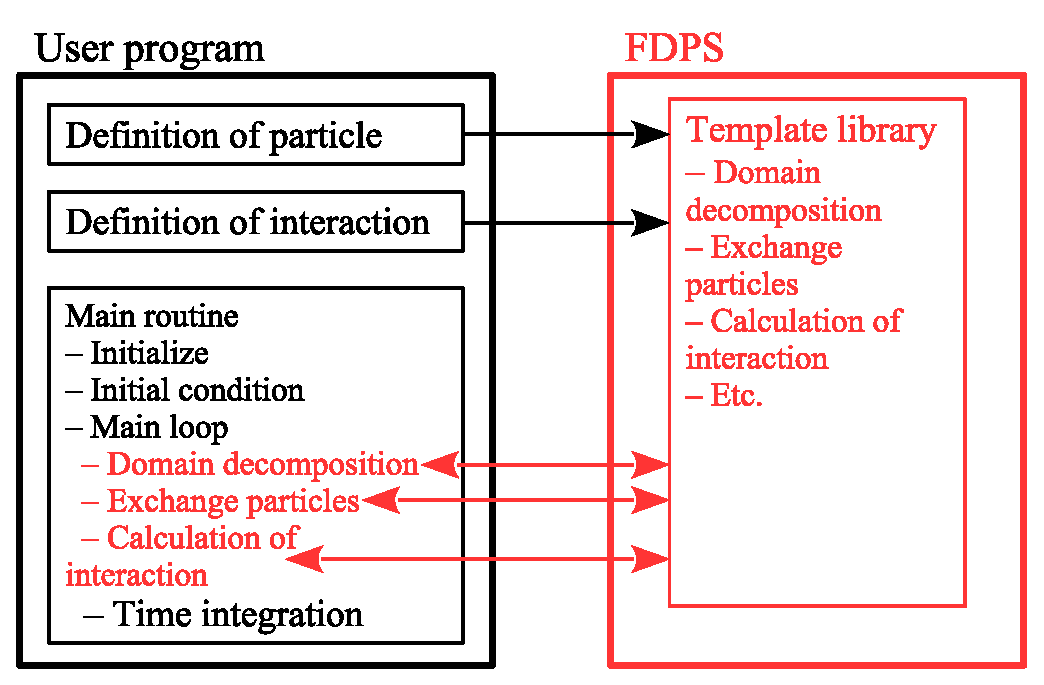
\includegraphics[width=8cm]{fig/concept.eps}
  \end{center}
  \caption{概念図}
  \label{fig:concept}
\end{figure}

%%%%%%%%%%%%%%%%%%%%%%%%%
\subsection{Sample code}

この節ではサンプルコードを示す。ここでは、アプリケーションとして重力N体
シミュレーションを用いる。

重力N体シミュレーションを式(\ref{eq:geq})に当てはめると以下のようになる。
\begin{align}
  \bm{u}_i &= (m_i, \bm{r}_i, \bm{v}_i) \\
%%
  \bm{f}(\bm{u}_i, \bm{u}_j) &= \left( 0, 0, \frac{G m_j (\bm{r}_j -
    \bm{r}_i)}{(|\bm{r}_j-\bm{r}_i|^2+\epsilon_i^2)^{3/2}} \right) \\
%%
  \bm{g}(\bm{u}_i) &= (0, \bm{v}_i, 0)
\end{align}
ここで、$G$は重力定数、$m_i$、$\bm{r}_i$、$\bm{v}_i$はそれぞれ粒子の質
量、位置、速度、$\epsilon_i$は粒子固有の重力ソフトニングである。

重力は無限遠まで到達する長距離力である。そのため、遠くの複数の粒子は超
粒子として1つにまとめる。このサンプルコードでは、超粒子を複数の粒子の
モノポールとして近似する。このとき、式(\ref{eq:geq})の第1項は以下のよ
うに近似できる。
\begin{align}
  \sum_j^N \bm{f}(\bm{u}_i,\bm{u}_j) \sim \sum_j^{N_\textbf{J}}
  \bm{f}(\bm{u}_i,\bm{u}_j) + \sum_s^{N_\textbf{S}}
  \bm{f}(\bm{u}_i,\bm{\hat{u}}_s)
\end{align}
ここで、$N_{\rm J}$は$i$粒子に作用する粒子の数、$N_{\rm S}$は$i$粒子に
作用する超粒子の数、$\bm{\hat{u}}_s$は超粒子の物理量ベクトルである。物
理量ベクトルの質量を超粒子をなす粒子の全質量、位置を超粒子をなす粒子の
重心とおけば、超粒子から$i$粒子への作用は、粒子から$i$粒子への作用と同
様の関数で記述できる。一般に、ユーザーは、粒子から粒子への作用の関数に
加え、超粒子から粒子への作用の関数を記述する必要があるが、ここでは必要
ない。

このN体シミュレーションをFDPSを使って実装すると、ソースコード
\ref{code:samplecode}のようになる。このコードをコピー\&ペーストして、
C++コンパイラまたはMPI対応のC++コンパイラでコンパイルすれば、ただちに動
作する。さらに、このコードは世界最高レベルの性能を持つ。FDPSを使えば、
このようなコードが120行足らずで書くことができるのである。

このサンプルコードは4つの部分からなる。すなわち、FDPSのインストール、
粒子を定義する部分、相互作用を定義する部分、メインルーチンとそこで呼出
される関数の定義である。以下、それぞれについて記述する。

1行目から2行目でFDPSのインストールを行っている。これはヘッダファイル
particle\_simulator.hppをインクルードするだけですむ。FDPSが提供するAPI
やクラスは名前空間PSで囲まれている。ここでは``using namespace PS''とし
て名前空間の明示を省略できるようにした。%%F64, F64vec

4行目から35行目では粒子、すなわち$\bm{u}_i$を定義している。この粒子は、
質量、ソフトニング長、位置、速度、加速度の情報を持つ。メンバ関数getPos、
getCharge、copyFromFP、clear、readAsciiはFDPSのライブラリとのデータの入
出力を定義するものである。メンバ関数predict、correctはメインルーチンの
中で粒子の軌道の時間積分を行うときに用いる。

37行目から61行目では相互作用の関数、すなわち$\bm{f}$の定義をしている。
この関数の引数を見ると、$i$粒子の配列ip、$i$粒子数ni、$j$粒子または超粒
子の配列jp、$j$粒子数nj、結果を受け取る配列forceがある。前述したように、
$j$粒子から$i$粒子への作用の形と超粒子から$i$粒子への作用の形は同じであ
る。そのため、この関数をテンプレート関数とし、引数に$j$粒子だけでなく超
粒子も取れるようにしている。この関数の中では、for文の2重ループを使って、
ni個の$i$粒子に対するnj個の$j$粒子または超粒子の作用を計算している。

並列処理以外のところでも、ユーザーが高性能化を意識しなくて済むように配
慮がなされている。相互作用の関数を定義する際には、複数の$i$粒子に対して
複数の$j$粒子が作用するという形で定義する。このとき$i$粒子、$j$粒子とも
に配列の形で与えられている。そのため単純なfor文による二重ループを記述す
ればよい。この配列は連続したメモリ上にメモリ確保されているため、単純な
二重ループさえ書けば、キャッシュヒット率が非常に高い。また、ユーザーが
ループ内をSIMD化するのも容易である。この配列が与えられるのは、各スレッ
ドでの上でのことなので、マルチスレッドについても意識する必要がない。

残りの部分では、メインルーチンとそこで呼び出される関数を定義している。
main関数は6つの部分に分かれている。すなわち以下の通りである。
\begin{itemize}
\item 時刻の初期化(92から94行目)
\item FDPSの初期化と終了(95と115行目)
\item FDPSが提供するテンプレートライブラリのオブジェクトの生成と初期化
  (96から102行目)
\item 粒子情報のファイルからの入力(103行目)
\item 初期の重力の計算(104から106行目)
\item リープフロッグ法を用いた常微分方程式の時間発展(107から114行目)
\end{itemize}
以下、2、3、4、5番目について詳述する。1番目は自明であるし、6番目
は時間積分の部分を除けば5番目の繰り返しである。

FDPSの初期化はMPIの初期化とOpenMPの初期化を行っており、FDPSの終了はMPI
の終了を行っている。FDPSのテンプレートライブラリを使用するのは、この初
期化と終了の間である必要がある。

次に行っているのはFDPSが提供するテンプレートライブラリのオブジェクトの
生成と初期化である。このライブラリはDomainInfoクラス、ParticleSystemク
ラス、TreeForForceクラスとして実装されている。それぞれのクラスのオブジェ
クトが持つ情報とAPIについて以下に記す。
\begin{itemize}
\item DomainInfoクラス: 全プロセスに割当てられた計算領域の情報を持ち、
  計算領域の分割を行うメソッドのAPIを持つ。
\item ParticleSystemクラス: 各プロセスの担当粒子の情報を持ち、プロセス
  間で粒子情報を交換するメソッドのAPIを持つ。このクラスはユーザーが定義
  する粒子クラスをテンプレート引数とするテンプレートクラスになっている。
\item TreeForForceクラス: 相互作用計算を高速にするためのツリー構造をデー
  タとして持ち、相互作用計算を行うメソッドのAPIを持つ。オブジェクトを生
  成する際に、計算する力のタイプ(TreeForForce``Long'')、計算すべき相互
  作用の情報と相互作用を計算するのに必要な$i$粒子の情報と相互作用を計算
  するのに必要な$j$粒子の情報(テンプレート第1、2、3引数)、相互作用を
  計算するのに必要な超粒子の情報(``Monopole'')を指定する。ここでは、テ
  ンプレート第1、2、3引数がすべて``Nbody''であるが、通信量の削減のた
  めに、それぞれのためにクラスを定義してテンプレート引数にすることが可
  能である。
\end{itemize}

オブジェクトptclへの粒子情報のファイルからの入力がメソッド
readParticleAsciiによってなされる。この引数argv[1]はコマンドライン上で
実行する際の第一引数のことである。このAPIの中で粒子クラスで定義した
readAsciiが呼出され、実際に粒子にデータが入力される。

各粒子への重力が計算される。これは関数calcGravAllAndWriteBackで実行され
る。この関数はmain関数の前に定義されている。以下、この関数の手順を説明
する。各手順は、2.1節の手順に対応する。
\begin{enumerate}
\item ロードバランスを以下の2ステップで取る。
  \begin{enumerate}
  \item 計算領域が分割される。これはオブジェクトdinfoのメソッド
    decomposeDomainAllが呼び出されて実行される。粒子分布が反映されるた
    め、オブジェクトptclが引数となる。
  \item 分割した計算領域に合せて、プロセス間で粒子情報が交換される。こ
    れはオブジェクトptclのメソッドexchangeParticleが呼出されて実行され
    る。全プロセスが担当する領域の情報が必要なので、オブジェクトdinfoが
    引数となる。
  \end{enumerate}
\item 相互作用を計算する。これはオブジェクトtreeのメソッド
  calcForceAllAndWriteBackが呼出されて実行される。この中で相互作用を計
  算する関数を呼出すため、第1、2引数に$j$粒子から$i$粒子への作用と超
  粒子から$i$粒子への作用を計算する関数CalcGravがある。$j$粒子と超粒子
  の指定はテンプレート引数によってなされ、それぞれNbodyとSPJMonopoleと
  なっている。SPJMonopoleはFDPSが提供する超粒子のクラスである。また、相
  互作用の計算には、粒子情報と領域情報も必要なため、第3引数にオブジェ
  クトptcl、第4引数にオブジェクトdinfoがある。
\end{enumerate}

In this section, we present the complete working example of a
simulation code written using FDPS, to illustrate how a user actually
uses FDPS. As the target problem, we use the gravitational $N$-body
problem with an open boundary.  Within the terminology of FDPS, the
interaction between particles in the gravitational $N$-body problem is
of the ``long-range'' type. Therefore, we need to specify the function
to calculate interactions for both the ordinary particles and
superparticles. For the sake of brevity, we use the center-of-mass
approximation for superparticles, which means we can actually use the
same function for both types of particles.

The physical quantity vector $\myvec{u}_i$ and interaction functions
$\myvec{f}$, $\myvec{f'}$, and $\myvec{g}$ for the gravitational
$N$-body problem is now given by:
\begin{align}
  \myvec{u}_i &= (\myvec{r}_i,
  \myvec{v}_i,m_i) \label{eq:PhysicalVectorNbody} \\
%%  
  \myvec{f} (\myvec{u}_i, \myvec{u}_j) &= \frac{Gm_j \left(
    \myvec{r}_j - \myvec{r}_i \right)}{ \left( |\myvec{r}_j -
    \myvec{r}_i|^2 + \epsilon_i^2
    \right)^{3/2}} \label{eq:ParticleParticleNbody} \\
%%
  \myvec{f'} (\myvec{u}_i, \myvec{u'}_j) &= \frac{Gm_j' \left(
    \myvec{r}_j - \myvec{r'}_i \right)}{ \left( |\myvec{r}_j -
    \myvec{r'}_i|^2 + \epsilon_i^2
    \right)^{3/2}} \label{eq:ParticleSuperparticleNbody} \\
%%
  \myvec{g}(\myvec{F},\myvec{u}_i)  &= (\myvec{v}_i,\myvec{F},0),
\label{eq:ConversionNbody}
\end{align}
where $m_i$, $\myvec{r}_i$, $\myvec{v}_i$, and $\epsilon_i$ are, the
mass, position, velocity, and gravitational softening of particle $i$,
$m_j'$ and $\myvec{r'}_j$ are, the mass and position of a
superparticle $j$, and $G$ is the gravitational constant.  Note that
the shapes of the functions $\myvec{f}$ and $\myvec{f'}$ are the same.

Listing~\ref{code:samplecode} shows the complete code which can be
actually compiled and run, not only on a single-core machine but also
massively-parallel, distributed-memory machines such as the full-node
configuration of the K computer. The total number of lines is only
117.


\begin{lstlisting}[label=code:samplecode,numbers=left,numbersep=5pt,frame=single,basicstyle=\ttfamily,caption=A sample code of $N$-body simulation]
#include <particle_simulator.hpp>
using namespace PS;

class Nbody{
public:
    F64    mass, eps;
    F64vec pos, vel, acc;
    F64vec getPos() const {return pos;}
    F64 getCharge() const {return mass;}
    void copyFromFP(const Nbody &in){ 
        mass = in.mass;
        pos  = in.pos;
        eps  = in.eps;
    }
    void copyFromForce(const Nbody &out) {
        acc = out.acc;
    }    
    void clear() {
        acc = 0.0;
    }
    void readAscii(FILE *fp) {
        fscanf(fp,
               "%lf%lf%lf%lf%lf%lf%lf%lf",
               &mass, &eps,
               &pos.x, &pos.y, &pos.z,
               &vel.x, &vel.y, &vel.z);
    }
    void predict(F64 dt) {
        vel += (0.5 * dt) * acc;
        pos += dt * vel;
    }
    void correct(F64 dt) {
        vel += (0.5 * dt) * acc;
    }
};

template <class TPJ>
struct CalcGrav{
    void operator () (const Nbody * ip,
                      const S32 ni,
                      const TPJ * jp,
                      const S32 nj,
                      Nbody * force) {
        for(S32 i=0; i<ni; i++){
            F64vec xi  = ip[i].pos;
            F64    ep2 = ip[i].eps
                * ip[i].eps;
            F64vec ai = 0.0;
            for(S32 j=0; j<nj;j++){
                F64vec xj = jp[j].pos;
                F64vec dr = xi - xj;
                F64 mj  = jp[j].mass;
                F64 dr2 = dr * dr + ep2;
                F64 dri = 1.0 / sqrt(dr2);                
                ai -= (dri * dri * dri
                       * mj) * dr;
            }
            force[i].acc += ai;
        }
    }
};

template<class Tpsys>
void predict(Tpsys &p,
             const F64 dt) {
    S32 n = p.getNumberOfParticleLocal();
    for(S32 i = 0; i < n; i++)
        p[i].predict(dt);
}

template<class Tpsys>
void correct(Tpsys &p,
             const F64 dt) {
    S32 n = p.getNumberOfParticleLocal();
    for(S32 i = 0; i < n; i++)
        p[i].correct(dt);
}

template <class TDI, class TPS, class TTFF>
void calcGravAllAndWriteBack(TDI &dinfo,
                             TPS &ptcl,
                             TTFF &tree) {
    dinfo.decomposeDomainAll(ptcl);
    ptcl.exchangeParticle(dinfo);    
    tree.calcForceAllAndWriteBack
        (CalcGrav<Nbody>(),
         CalcGrav<SPJMonopole>(),
         ptcl, dinfo);    
}

int main(int argc, char *argv[]) {
    F32 time  = 0.0;
    const F32 tend  = 10.0;
    const F32 dtime = 1.0 / 128.0;
    PS::Initialize(argc, argv);
    PS::DomainInfo dinfo;
    dinfo.initialize();
    PS::ParticleSystem<Nbody> ptcl;
    ptcl.initialize();
    PS::TreeForForceLong<Nbody, Nbody,
        Nbody>::Monopole grav;
    grav.initialize(0);
    ptcl.readParticleAscii(argv[1]);
    calcGravAllAndWriteBack(dinfo,
                            ptcl,
                            grav);
    while(time < tend) {
        predict(ptcl, dtime);        
        calcGravAllAndWriteBack(dinfo,
                                ptcl,
                                grav);
        correct(ptcl, dtime);        
        time += dtime;
    }
    PS::Finalize();
    return 0;
}
\end{lstlisting}


Now let us explain how this sample code works. This code consists of
four parts: The declaration to use FDPS (lines 1 and 2), the
definition of the particle (the vector $\myvec{u}_i$) (lines 4 to 35),
the definition of the gravitational force (the functions $\myvec{f}$
and $\myvec{f'}$) (lines 37 to 61), and the actual user program,
comprising a user-defined main routine and user-defined functions from
which library functions of FDPS are called (lines 63 to line 117). In
the following, we explain them step by step.

In order to declare to use FDPS, the only thing the user program need
to do is to include the header file ``particle\_simulator.hpp''. This
file and other source library files of FDPS should be in the include
path of the compiler. Everything in the standard FDPS library is
provided as the header source library, since they are implemented as
template libraries which need to receive particle class and
interaction functions. Everything in FDPS is provided in the namespace
``PS''. Therefore in this sample program, we declare it as the default
namespace to simplify the code. (For simplicity's sake, we do not omit
the namespace ``PS'' of FDPS functions and class templates in the main
routine.)

Before going to the 2nd parts, let us list the data types and classes
defined in FDPS. \texttt{F32/F64} are data types of 32-bit and 64-bit
floating points. \texttt{S32} is a data type of 32-bit signed integer.
\texttt{F64vec} is a class of a vector consisting of three 64-bit
floating points. This class provides several operators, such as the
addition, subtraction and the inner product indicated by ``$*$''.
Users need not use these data types in their own program, but some of
the functions which users should define should return the values in
these data types.

In the 2nd part, we define the particle, i.e. the vector
$\myvec{u}_i$, as a class \texttt{Nbody}. This class has member
variables: \texttt{mass} ($m_i$), \texttt{eps}
($\epsilon_i$), \texttt{pos} ($\myvec{r}_i$), \texttt{vel}
($\myvec{v}_i$), and \texttt{acc} ($d\myvec{v}_i/dt$). Although the
member variable \texttt{acc} does not appear in
equation~(\ref{eq:PhysicalVectorNbody}) -- (\ref{eq:ConversionNbody}),
we need this variable to store the result of the gravitational force
calculation. A particle class for FDPS must provide public member
functions \texttt{getPos}, \texttt{getCharge}, \texttt{copyFromFP},
\texttt{copyFromForce}, \texttt{clear},
and \texttt{readAscii}, in these names, so that the internal functions
of FDPS can access the data within the particle class.  For the name
of the particle class itself and the names of the member variables, a
user can use whatever names allowed by the C++ syntax.  The member
functions \texttt{predict} and \texttt{correct} are used in the
user-defined part of the code to integrate the orbits of particles.
Note that since the interaction used here is of $1/r$ type, the
definition and construction method of the superparticle are given as
the default in FDPS and not shown here.

In the 3rd part, the interaction functions $\myvec{f}$ and
$\myvec{f'}$ are defined. Since the shapes of the functions
$\myvec{f}$ and $\myvec{f'}$ are the same, we give one as a template
function.  The interaction function used in FDPS should have the
following five arguments. The first argument \texttt{ip} is the
pointer to the array of variables of particle
class \texttt{Nbody}. This argument specifies $i$-particles which
receive the interaction. The second argument \texttt{ni} is the number
of $i$-particles. The third argument \texttt{jp} is the pointer to the
array of variable of a template data type \texttt{TPJ}. This argument
specifies $j$-particles or superparticles which exert the
interaction. The fourth argument \texttt{nj} is the number of
$j$-particles or super-particles. The fifth argument \texttt{force} is
the pointer to the array of a variable of a user-defined class to
which the calculated interaction on an $i$-particle can be stored. In
this example, we used the particle class itself, but this can be
another class or a simple array.

%
The interaction function should be defined as a function object, so
that it can be passed to other functions as argument. Thus, it is
declared as a \texttt{struct}, with the only member
function \texttt{operator ()}.  In this example, the interaction is
calculated through a simple double loop. In order to make full
advantage of the SIMD unit in modern processors,
architecture-dependent tuning may be necessary, but only to this
single function.

In the 4th part, we give the main routine and functions called from
the main routine. In the following, we describe the main routine in
detail, and briefly discuss other functions. The main routine consists
of the following seven steps:
\begin{enumerate}
\item Set simulation time and timestep (lines 92 to 94). \label{proc:literal}
\item Initialize FDPS (line 95). \label{proc:init}
\item Create and initialize objects of FDPS classes (lines 96 to 102). \label{proc:construct}
\item Read in particle data from a file (line 103). \label{proc:input}
\item Calculate the gravitational forces of all the particles at the
  initial time (lines 104 to 106). \label{proc:calcinteraction}
\item Integrate the orbits of all the particles with Leap-Frog method
  (lines 107 to 114). \label{proc:integration}
\item Finish the use of  FDPS (line 115). \label{proc:fin}
\end{enumerate}

In the following, we describe  steps~\ref{proc:init},
\ref{proc:construct}, \ref{proc:input}, \ref{proc:calcinteraction},
and \ref{proc:fin}, and skip steps~\ref{proc:literal}
and \ref{proc:integration}.  In step~\ref{proc:literal}, we do not
call FDPS libraries.  Although we call FDPS libraries in
step~\ref{proc:integration}, the usage is the same as in
step~\ref{proc:calcinteraction}.

In step~\ref{proc:init}, the FDPS function \texttt{Initialize} is
called. In this function, MPI and OpenMP libraries are initialized. If
neither of them are used, this function does nothing.  All functions
of FDPS must be called between this function and the
function \texttt{Finalize}.

In step~\ref{proc:construct}, we create and initialize three objects
of the FDPS classes:
\begin{itemize}
\item \texttt{dinfo}: An object of class \texttt{DomainInfo}. It is
  used for domain decomposition.
\item \texttt{ptcl}: An object of class template \texttt{ParticleSystem}.
It takes the user-defined particle class (in this
example, \texttt{Nbody}) as the template argument. From the user
program, this object looks as an array of $i$-particles.
\item \texttt{grav}: An object of a data type \texttt{Monopole} defined in
a class template \texttt{TreeForForceLong}. This object is used for
the calculation of long-range interaction using the tree algorithm.
It receives three user-defined classes template arguments: the class
to store the calculated interaction, the class for $i$-particles and
the class for $j$-particles. In this example, all three are the same
as the original class of particles.  It is possible to define classes
with minimal data for these purposes and use them here, in order to
optimize the cache usage. The data type \texttt{Monopole} indicates
that the center-of-mass approximation is used for superparticles.
\end{itemize}

In step~\ref{proc:input}, the data of particles are read from a file
into the object \texttt{ptcl}, using the FDPS
function \texttt{readParticleAscii}. In the function, a member
function of class \texttt{Nbody}, \texttt{readAscii}, is called.

In step~\ref{proc:calcinteraction}, the forces on all particles are
calculated through the function \texttt{calcGravAllAndWriteBack}, which
is defined in lines 79 to 89. In this function,
steps~\ref{proc:decompose}, \ref{proc:exchange}, and
\ref{proc:interaction} in section~\ref{sec:view} are performed. In
other words, all of the actual work of FDPS libraries to calculate
interaction between particles takes place here. For
step~\ref{proc:decompose}, \texttt{decomposeDomainAll}, a member function
of class \texttt{DomainInfo} is called. This function takes the object
\texttt{ptcl} as an argument to use the positions of particles to
determine the domain decomposition.  Step~\ref{proc:exchange} was
performed in \texttt{exchangeParticle}, a member function of
class \texttt{ParticleSystem}. This function takes the
object \texttt{dinfo} as an argument and redistributes particles among
MPI processes.  Step~\ref{proc:interaction} was performed
in \texttt{calcForceAllAndWriteBack}, a member function of
class \texttt{TreeForForceLong}. This function takes the user-defined
function object \texttt{CalcGrav} as the first and second arguments,
and calculates particle-particle and particle-superparticle
interactions using them.

In step~\ref{proc:fin}, the FDPS function \texttt{Finalize} is
called. It calls the \texttt{MPI\_finalize} function.

In this section, we have described in detail how a user program
written using FDPS looks like. As we stated earlier, this program can
be compiled with or without parallelization using MPI and/or OpenMP,
without any change in the user program. The executable parallelized
with MPI is generated by using an appropriate compiler with MPI
support and a compile-time flag.  Thus, a user need not worry about
complicated bookkeeping necessary for parallelization using MPI.
%
In the next section, we describe how FDPS provides a generic
framework which takes care of parallelization
and bookkeeping for particle-based simulations. 

% LocalWords:  monopole superparticle FDPS hpp namespace nd th vec Nbody eps dt
% LocalWords:  pos vel acc getPos getCharge copyFromFP copyFromForce readAscii
% LocalWords:  ip const ni jp TPJ nj MPI OpenMP DomainInfo dinfo subdomains
% LocalWords:  subdomain ParticleSystem ptcl TreeForForceLong readParticleAscii
% LocalWords:  calcGravAllAndWriteBack decomposeDomainAll exchangeParticle SIMD
% LocalWords:  calcForceAllAndWriteBack CalcGrav superparticles struct grav
% LocalWords:  parallelization parallelized timestep


%%%%%%%%%%%%%%%%%%%%%%%%%%%%%%%%%%%%%%%%%%%%%%%%%%%%%
\section{Implementation}

この節ではFDPSの中の実装について述べる。FDPSの中では分散メモリ環境での
並列処理にはMPIを用い、共有メモリ環境での並列処理にはOpenMPを用いている。
これらを用いるのはこれらのポータビリティが高いためである。この節で具体
的に扱うのは、FDPS内で行われているロードバランスの実装と相互作用計算の
実装である。以下では、この順に記述する。

\subsection{ロードバランス}

FDPSでは、計算時間がプロセスの間で均等になるように、ロードバランスを取
る。これは、計算領域を分割して各プロセスに割り当て、各プロセスは担当領
域内にある粒子の時間発展を追うのに責任を持つ、という形で実現される。

計算領域の分割の仕方は、3-dimensional multi-section decompositionと呼ば
れる方法である。この方法では、まず計算領域をx軸に垂直な面でnx個に分割、
今度は各領域をy軸に垂直な面でny個に分割、最後に各領域をz軸に垂直な面で
nz 個に分割するというものである。従って、各プロセスが担当する領域は直方
体となる。領域分割した結果は図を参照。nx, ny, nzの決め方には自由度があ
るが、なるべくnx, ny, nzの値が等しくなるようにする。このようにするのは
相互作用計算などをする際に交換する粒子の数を少なくできるからである。

他にも良い分割方法はある。しかし、FDPSの方法が他の方法に比べて実装がシ
ンプルである。また、シンプルであるのにも関わらず、ロードバランスも悪く
ない。

以下、ロードバランスの実装方法について述べる。ロードバランスは領域分割
と粒子交換の2ステップに分かれる。これらはFDPSが提供するDomainInfoクラ
スのメソッドdecomposeDomainAllとParticleSystemクラスのメソッド
exchangeParticleに対応する。

まず領域分割の実装方法について述べる。FDPSではサンプリング法という方法
を採用している。この方法では、各プロセスから粒子をサンプルし、それらの
粒子の空間分布から領域の分割の仕方を決定するものである。全粒子の空間分
布から決定するよりもランダムノイズは入りやすいが、扱う粒子数が小さいた
めに計算コストを小さくできる。FDPSでは、ランダムノイズを抑えるために、
現ステップのサンプル粒子から決めた領域情報から領域分割をするのではなく、
1ステップ前の領域情報も使って、現ステップの領域情報を決定する。

以下、領域分割の手順を記述する。
\begin{enumerate}
\item 各プロセスが自分の担当粒子からランダムに粒子をサンプルする。全プ
  ロセスでサンプルする粒子数はプロセス数に比例した数である。各プロセス
  でサンプルする粒子数は、全プロセスでサンプルする粒子数にある割合をか
  けたもので決まる。この割合を決定するのはユーザーであるが、適切なロー
  ドバランスを取るには、各プロセスで前のステップにかかった計算時間を前
  のステップでかかった全プロセスの計算時間の和で割ったものなどがよい。
\item 各プロセスがそれぞれのサンプル粒子の数をMPI\_Allgatherを用いてラ
  ンク0のプロセスに集め、その後、各プロセスがそれぞれのサンプル粒子の位
  置情報をMPI\_Allgathervを用いてランク0のプロセスに集める。
\item 以下3つのサブステップで暫定的な領域分割を行う。ここでは1プロセス
  だけがソートを行うが、あまり計算時間はかからない。ソートするのはサン
  プル粒子なので、数が少ないからである。
  \begin{enumerate}
  \item ランク0のプロセスで、サンプル粒子をそれらのx座標でソートし、サ
    ンプル粒子がx軸方向にnx等分されるようにx軸に垂直な面で空間を分割す
    る。
  \item ランク0のプロセスで、上で分割した各領域のサンプル粒子をy座標で
    ソートし、サンプル粒子がy軸方向にny等分されるようにy軸に垂直な面で
    空間を分割する。
  \item ランク0のプロセスで、上で分割した各領域のサンプル粒子をz座標で
    ソートし、サンプル粒子がz軸方向にnz等分されるようにz軸に垂直な面で
    空間を分割する。
  \end{enumerate}
\item 上で求めた暫定的な領域情報と現在の領域情報を用いて、指数移動平均
  を行い、領域情報を決定する。これは領域分割に全粒子の空間情報ではなく、
  サンプルした粒子の空間情報を決めることによるランダムノイズを小さくす
  るために行う。
\item MPI\_Bcastを用いて、ランク0のプロセスが、分割した領域の情報を他の
  すべてのプロセスに放送する。
\end{enumerate}

次に粒子交換の実装方法について述べる。これは以下のような手順で実行され
る。
\begin{enumerate}
\item 各プロセスが、自分の担当粒子のうち自分の担当領域からはみでている
  粒子を探す。ここでは、いきなり担当粒子すべての行先を探すということは
  しない。前のタイムステップでロードバランスが取られていれば、自分の担
  当領域からはみでている粒子はあまり多くないし、行先を探すコストは大き
  いからである。
\item 各プロセスが、自分の担当領域からはみでている粒子すべての送り先の
  プロセスを探す。ここでは、各粒子の位置と他のすべてのプロセスの担当領
  域を比較する、というようなことはしない。それよりも、まずx軸方向で一致
  するプロセス群を探し、その後y軸方向で一致するプロセス群を探し、最後に
  z軸方向で一致するプロセスを探す。前者の計算コストは$\mathcal{O}(p)$で
  あるが、後者の計算コストは$\mathcal{O}(3p^{1/3})$である。プロセス数が
  10を越えれば、確実に後者の計算コストの方が小さい。
\item MPI\_Alltoallを呼び、送りつける粒子の数を交換し、その後
  MPI\_Alltoallvを呼び、粒子情報を交換する。
\end{enumerate}

\subsection{相互作用計算}

相互作用の計算は、TreeForForceクラスのメソッドcalcForceAllAndWriteBack
によって実行される。この中では、各プロセスが担当する粒子の相互作用の計
算に必要な粒子の情報を他のプロセスから集め、ユーザーが定義した相互作用
を計算する関数を呼び出し、相互作用を計算する。以下では、この実装につい
て記述する。

このメソッドは以下の3ステップを実行する。
\begin{enumerate}
\item 各プロセスが全担当粒子の相互作用の計算に必要な粒子の情報を他のプ
  ロセスから集める。
\item 各プロセスが担当粒子それぞれの相互作用の計算に必要な粒子のリスト
  を作る。
\item 相互作用の計算をする。
\end{enumerate}
このうちの最後のステップはユーザーの定義する関数の中で行われるため、実
装はユーザーに任される。従って、以下では最初と2番目のステップの実装を
記述する。

まず、各プロセスが担当粒子の相互作用計算に必要な粒子を他のプロセスから
集める方法を述べる。これは、基本的には、octree structureを用いたBHツリー
アルゴリズムや近傍粒子探査法の並列版である。BHツリーアルゴリズムは力が
長距離力の場合に、近傍粒子探査法は力が短距離力の場合に、用いられる。厳
密にいえば、それぞれの方法には若干の違いがあるが、ここではその違いには
深く立ち入らずに記述する。

以下、その手順を記述する。
\begin{enumerate}
\item $i$プロセスで担当粒子すべてからなるoctree構造を構築する。この
  octree 構造をローカルツリーと呼ぶ。
\item $i$プロセスがローカルツリーの各ツリーセルのモーメントを計算する。
  このモーメントは長距離力ならばこのツリーセルに含まれる粒子すべての多
  重極モーメントであり、短距離力ならばこのツリーセルに含まれる粒子の探
  査半径の最大値である。
\item $i$プロセスが自分の担当粒子にとって必要な$j$プロセスの担当粒子を
  集める。これは次のようなステップで行われる。
  \begin{enumerate}
  \item $i$プロセスが、自分のローカルツリーを使い、自分の担当粒子のうち
    $j$プロセスの担当粒子を必要とする粒子を探し、$j$プロセスに自分の担
    当粒子を送る。また$j$プロセスから、$j$プロセスの担当粒子のうち$i$プ
    ロセスの担当粒子を必要とする粒子を受け取る。このステップは力の影響
    範囲が、$i$粒子固有の探査半径で決まっていない場合にはスキップできる。
    この場合、$i$プロセスと$j$プロセスの位置関係だけで、$i$プロセスの担
    当粒子にとって必要な$j$プロセスの担当粒子が決まるからである。
  \item $i$プロセスが、自分のローカルツリーを使って、$j$プロセスにとっ
    て必要な自分の担当粒子を探す。
  \item $i$プロセスが$j$プロセスにとって必要な自分の担当粒子を送り、
    $j$プロセスからは$i$プロセスにとって必要な$j$プロセスの担当粒子を受
    け取る。
  \end{enumerate}
\item $i$プロセスは自分の担当粒子すべてと他のプロセスから受け取ったすべ
  ての粒子からなるoctree構造を構築する。このoctree構造をグローバルツリー
  と呼ぶ。
\item $i$プロセスがグローバルツリーの各ツリーセルのモーメントを計算する。
\end{enumerate}

次に、各プロセスが担当粒子の相互作用の計算に必要な粒子のリストを作成す
について述べる。このリストは複数の$i$粒子に対する共通のリストである。こ
のようなリストを作るのは、ユーザーが相互作用関数を作る際、キャッシュヒッ
ト率の向上を意識する必要がなく、またSIMD化もしやすいからである。

以下、リスト作成の手順を述べる。
\begin{enumerate}
\item 各プロセスの各スレッドが、作用する粒子のリストを共有する$i$粒子の
  グループを作る。この$i$粒子のグループは、粒子数$n_{\rm group}$を上限
  とするツリーセルに属するすべての粒子から構成される。
\item 各プロセスの各スレッドが、グローバルツリーを使って、$i$粒子のグルー
  プに作用する粒子のリストを作る。この粒子リストは連続するメモリに格納
  される。相互作用計算の際のキャッシュヒット率を高くするためである。
\end{enumerate}
各リストが各スレッドで作成されるために、相互作用関数は各スレッドで動作
することになっている。従って、ユーザーが相互作用関数を作成する際に
OpenMPを意識する必要がない。

%%%%%%%%%%%%%%%%%%%%%%%%%%%%%%%%%%%%%%%%%%%%%%%%%%%%%
\section{Performance}

\underbold{組込むべき言葉}
\begin{itemize}
\item 使用した計算機のピーク性能、アプリのピーク性能、アプリの実行性能
\end{itemize}

\begin{itemize}
\item N-body (スパイラル): 岩澤担当
  \begin{itemize}
  \item ベンチマーク(京、x86)
  \item エネルギーエラーがあったほうが後々役立つかも?
  \item きれいな絵
  \end{itemize}
\item std SPH (Giant Impact): 細野担当
  \begin{itemize}
  \item ベンチマーク(京、x86)
  \item きれいな絵
  \end{itemize}
\end{itemize}

\subsection{Gravitational $N$-body simulation}

\subsection{SPH simulation}

\begin{align}
  \frac{dm}{dt} &= 0 \\
%%
  \frac{d\bm{r}}{dt} &= \bm{v} \\
%%
  \frac{d\bm{v}}{dt} &= - \frac{\nabla p}{\rho} + \bm{g}
\end{align}

%%%%%%%%%%%%%%%%%%%%%%%%%%%%%%%%%%%%%%%%%%%%%%%%%%%%%
\section{Discussion and Conclusion}

%%%%%%%%%%%%%%%%%%%%%%%%%%%%%%%%%%%%%%%%%%%%%%%%%%%%%
\section{気になる文}

\begin{itemize}
\item C++プログラムから呼び出せる関数群からなるライブラリ
\item メッセージパッシングを用いたプログラムを設計、開発するのが非常に
  難しい
\item collective procedure
\item force calculation: the same way as in the case of the
  uniprocessor code
\item Time integration: sec. 3.4 Makino (2004)
\end{itemize}

\end{document}
